% Provenance (never printed): see sources/outline_sources.md (Year 1: heat sources,
% radiogenic and secular cooling; heat-flow measurement; the steady conductive geotherm
% with heat production; convection against conduction; the lithosphere as a thermal
% boundary layer). Curves from figdata/bachelor-1/geotherms.py; exercise and problem
% values in the Book 3 scratch calculator calc/ch10.py.
\chapter{De warmtebalans van de aarde}\label{ch:b1:heat-budget}

Onder een berg in de Japanse Alpen wacht in een oude mijngrot een tank met duizend ton vloeibare scintillator op zwakke lichtflitsen. De meeste komen van antineutrino's die in de kerncentrales van het omringende land worden gemaakt, maar sommige komen van onderaf: het uranium en thorium in de aarde zenden bij hun verval antineutrino's uit, en die gaan door de hele planeet heen alsof die leeg is. In 2135 dagen meten registreerde de detector 841 kandidaatgebeurtenissen, waarvan er 106 aan de aarde zelf werden toegeschreven. Uit die handvol flitsen schatte haar team in 2011 dat het verval van uranium en thorium de aarde met ongeveer 20 terawatt verwarmt. De planeet als geheel verliest er ongeveer 47. Dit hoofdstuk verklaart het verschil: waar de warmte van de aarde vandaan komt, hoe de warmte die naar buiten stroomt wordt gemeten, hoe de temperatuur met de diepte stijgt wanneer de warmte door geleiding wordt vervoerd, waarom de \omterm{def:b1:layered-earth:layers}{mantel} moet convecteren, en waarom de platen de koude bovenrand van die convectie vormen.

\begin{recall}
Warmte stroomt van warm naar koud; de warmtegeleidbaarheid $k$ van een gesteente meet hoe gemakkelijk warmte erdoorheen gaat, en de thermische diffusiviteit $\kappa = k/(\rho c)$ hoe snel een temperatuurverandering zich verspreidt (natuurkunde, tweede jaar universiteit). Radioactieve kernen vervallen met een vaste halveringstijd (natuurkunde). De temperatuur stijgt met de diepte langs de \omterm{def:b1:heat-budget:geotherm}{geotherm}, en de \omterm{def:b1:layered-earth:layers}{mantel} convecteert (Boek 2, klassen 11 en 12). De \omterm{def:b1:layered-earth:lithosphere}{lithosfeer} is de sterke buitenste schil van de aarde (\cref{ch:b1:layered-earth}).
\end{recall}

\section{Waar de warmte vandaan komt}

\begin{definition}[Warmtestroom]\label{def:b1:heat-budget:heat-flow}
De \emph{warmtestroom}\index{warmtestroom} $q$ op een punt van het aardoppervlak, of de warmtestroomdichtheid aan het oppervlak, is het vermogen van inwendige oorsprong dat daar per oppervlakte-eenheid door het oppervlak naar buiten stroomt, positief naar buiten gerekend. Zij wordt gemeten in \unit{W.m^{-2}}, in de praktijk in \unit{mW.m^{-2}}. Geïntegreerd over het hele oppervlak geeft zij het warmteverlies van de aarde $Q = \oint q\,\mathrm dS$.
\end{definition}

De \omterm{def:b1:heat-budget:heat-flow}{warmtestroom} is op tienduizenden plaatsen gemeten. Een compilatie van \num{38347} metingen, in 2010 gepubliceerd, geeft de gemiddelde waarden hieronder, met oceanen en continenten apart:
\begin{center}
\small
% ledger: dd10:split, dd10:total
\begin{tabular}{lccc}
\hline
 & oppervlak (\unit{m^2}) & warmteverlies (\unit{TW}) & gemiddelde \omterm{def:b1:heat-budget:heat-flow}{warmtestroom} (\unit{mW.m^{-2}}) \\
\hline
continenten & \num{2.073e14} & 14.7 & 70.9 \\
oceanen & \num{3.028e14} & 31.9 & 105.4 \\
hele aarde & \num{5.101e14} & 46.7 & 91.6 \\
\hline
\end{tabular}
\end{center}
Het totaal, afgerond op zijn onzekerheid, is $Q = \qty[uncertainty-mode=separate]{47 \pm 2}{TW}$. Twee derde ervan verlaat de aarde via de oceaanbodem, die jonger en dunner is dan de continenten. Het is een kleine stroom: de zon levert ongeveer \qty{173000}{TW} aan de aarde, en de inwendige warmte is \qty{0.03}{\percent} van de energiebalans aan het oppervlak. % ledger: nasa:solar-mean
Maar zij is de stroom die vulkanen, platen en bergvorming aandrijft, en zij heeft twee bronnen.

\begin{definition}[Radiogene warmteproductie]\label{def:b1:heat-budget:heat-production}
De \emph{radiogene warmteproductie}\index{radiogene warmteproductie} $A$ van een gesteente is de warmte die per volume-eenheid en per tijdseenheid vrijkomt door het verval van de radioactieve kernen die het bevat, in \unit{W.m^{-3}}, in de praktijk in
\unit{\micro W.m^{-3}}. Een gesteente met dichtheid $\rho$ dat massafracties $C_i$ bevat van de warmteproducerende elementen, die elk $H_i$ watt per kilogram element vrijmaken, heeft
\[
  A = \rho \sum_i C_i H_i .
\]
\end{definition}

Vier isotopen leveren bijna al deze warmte, omdat zij langlevend, overvloedig genoeg en energierijk zijn: \ce{^{238}U}, \ce{^{235}U}, \ce{^{232}Th} en \ce{^{40}K}. De warmte per kilogram van elk element is de warmte per kilogram van het radioactieve isotoop maal het aandeel van dat isotoop in het element (\cref{exo:b1:heat-budget:3}):
\begin{center}
\small
% ledger: dye:isotope-heat, iaea:isotopes
\begin{tabular}{lcccc}
\hline
isotoop & halveringstijd & warmte per kg isotoop & aandeel van het & warmte per kg element \\
 & (\unit{Gyr}) & (\unit{W.kg^{-1}}) & element (atomen) & (\unit{W.kg^{-1}}) \\
\hline
\ce{^{238}U} & 4.468 & \num{9.513e-5} & \qty{99.274}{\percent} & U: \num{9.85e-5} \\
\ce{^{235}U} & 0.704 & \num{5.685e-4} & \qty{0.720}{\percent} & \\
\ce{^{232}Th} & 14.0 & \num{2.628e-5} & vrijwel alles & Th: \num{2.63e-5} \\
\ce{^{40}K} & 1.248 & \num{2.847e-5} & \qty{0.0117}{\percent} & K: \num{3.40e-9} \\
\hline
\end{tabular}
\end{center}
Kalium geeft dertigduizend keer minder warmte per kilogram vrij dan uranium, maar het is een belangrijk element in veel gesteenten, uitgedrukt in procenten, terwijl uranium en thorium in delen per miljoen worden uitgedrukt. De gesteenten die rijk zijn aan alle drie zijn de graniet en verwante gesteenten; de armste zijn de peridotieten van de \omterm{def:b1:layered-earth:layers}{mantel}. Een compilatie van \num{2188} analyses geeft deze medianen, in \unit{\micro
W.m^{-3}}:
\begin{center}
\small
% ledger: vila:heat-production
\begin{tabular}{lclclc}
\hline
rhyoliet & 2.55 & slibgesteenten & 1.44 & gabbro & 0.35 \\
graniet & 2.43 & zandsteen & 0.82 & basalt & 0.21 \\
granodioriet & 1.88 & carbonaatgesteenten & 0.42 & ultramafische gesteenten & 0.11 \\
\hline
\end{tabular}
\end{center}
De spreiding binnen elke groep is groot: een kwart van de granieten produceert minder dan \qty{1.74}{\micro W.m^{-3}}, en een kwart meer dan \qty{3.23}{\micro W.m^{-3}}. De continentale \omterm{def:b1:layered-earth:layers}{korst} is verrijkt in deze elementen, de oceanische \omterm{def:b1:layered-earth:layers}{korst} en de \omterm{def:b1:layered-earth:layers}{mantel} zijn verarmd; maar de \omterm{def:b1:layered-earth:layers}{mantel} is zo groot dat zij nog steeds een groot deel van de warmtebronnen van de planeet bevat.

\begin{definition}[Seculiere afkoeling]\label{def:b1:heat-budget:secular-cooling}
\emph{Seculiere afkoeling}\index{seculiere afkoeling} is het deel van het warmteverlies van de aarde dat wordt geleverd door de langzame daling van de temperatuur van haar binnenste, \omterm{def:b1:layered-earth:layers}{mantel} en kern: het vrijkomen van warmte die sinds de vorming van de planeet is opgeslagen, met een snelheid $-\sum_j M_j c_j\,\mathrm dT_j/\mathrm dt$ voor reservoirs van massa $M_j$, soortelijke warmte $c_j$ en gemiddelde temperatuur $T_j$.
\end{definition}

Energiebehoud geeft de balans van de hele aarde: de warmte die aan het oppervlak verloren gaat is de radiogene productie plus de \omterm{def:b1:heat-budget:secular-cooling}{seculiere afkoeling},
\[
  Q = H_{\text{rad}} + Q_{\text{sc}} .
\]
De geoneutrino's meten een deel van de eerste term: het resultaat van 2011, dat twee detectoren combineerde, schrijft \qty{20}{TW} toe aan uranium en thorium, en \ce{^{40}K}, waarvan de antineutrino's te zwak zijn om zo te worden gedetecteerd, wordt geschat op ongeveer \qty{4}{TW}.
% ledger: kamland:2011
Ongeveer de helft van het warmteverlies is dus radiogeen, en de andere helft, ongeveer \qty{23}{TW}, is \omterm{def:b1:heat-budget:secular-cooling}{seculiere afkoeling}. Een deel van die afkoeling komt van de kern: de warmte die over de \omterm{def:b1:layered-earth:discontinuity}{kern-mantelgrens} stroomt, wordt geschat op \qtyrange{5}{15}{TW}. Deze getallen zijn onzeker: de meting zelf draagt een onzekerheid van ongeveer \qty{9}{TW}, en de geoneutrino-resultaten tot nu toe beperken het radiogene deel slechts tot \qtyrange{15}{41}{TW}, terwijl aardmodellen van verschillende soort lopen van \qtyrange{14}{46}{TW}. Het totaal, aan het oppervlak gemeten, is de best bekende term van de balans (figuur hieronder).
% ledger: dye:radiogenic

\begin{omfigure}
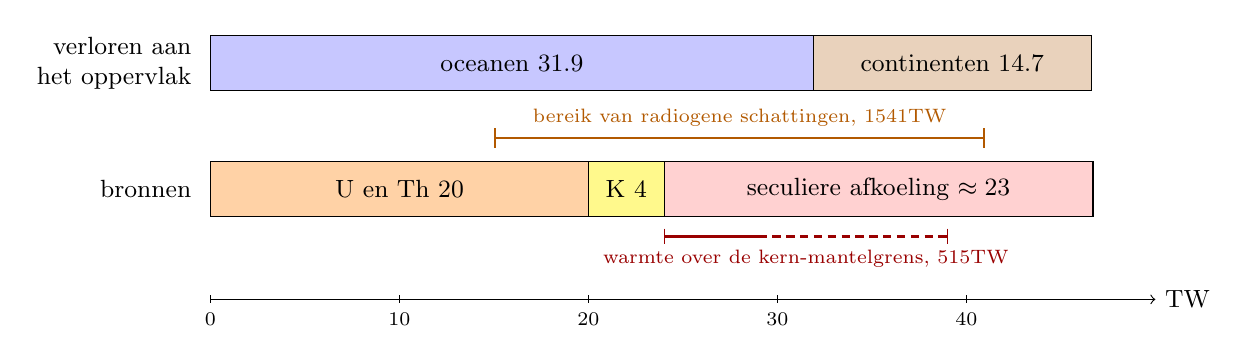
\begin{tikzpicture}[x=0.24cm, y=1cm, font=\small]
% ledger: dd10:split, kamland:2011, dye:radiogenic
% losses
\fill[blue!22] (0,1.6) rectangle (31.9,2.3);
\fill[brown!35] (31.9,1.6) rectangle (46.6,2.3);
\draw (0,1.6) rectangle (46.6,2.3);
\draw (31.9,1.6) -- (31.9,2.3);
\node at (15.95,1.95) {oceanen 31.9};
\node at (39.25,1.95) {continenten 14.7};
\node[anchor=east, align=right, font=\small] at (-0.5,1.95) {verloren aan\\het oppervlak};
% sources
\fill[orange!35] (0,0) rectangle (20,0.7);
\fill[yellow!45] (20,0) rectangle (24,0.7);
\fill[red!18] (24,0) rectangle (46.7,0.7);
\draw (0,0) rectangle (46.7,0.7);
\draw (20,0) -- (20,0.7) (24,0) -- (24,0.7);
\node at (10,0.35) {U en Th 20};
\node at (22,0.35) {K 4};
\node at (35.35,0.35) {seculiere afkoeling $\approx 23$};
\node[anchor=east, align=right] at (-0.5,0.35) {bronnen};
% core part of secular cooling (range)
\draw[red!60!black, very thick] (24,-0.25) -- (29,-0.25);
\draw[red!60!black, thick, densely dashed] (29,-0.25) -- (39,-0.25);
\draw[red!60!black] (24,-0.15) -- (24,-0.35) (39,-0.15) -- (39,-0.35);
\node[anchor=north, font=\scriptsize, red!60!black] at (31.5,-0.3) {warmte over de kern-mantelgrens, \qtyrange{5}{15}{TW}};
% radiogenic range
\draw[|-|, orange!70!black, thick] (15,1.0) -- (41,1.0);
\node[anchor=south, font=\scriptsize, orange!70!black] at (28,1.02) {bereik van radiogene schattingen, \qtyrange{15}{41}{TW}};
% axis
\draw[->] (0,-1.05) -- (50,-1.05) node[right] {TW};
\foreach \x in {0,10,20,30,40} {\draw (\x,-1.0) -- (\x,-1.1) node[below, font=\scriptsize] {\x};}
\end{tikzpicture}

\par\smallskip{\small De warmtebalans van de aarde. Boven: de warmte die door de oceaanbodem en de continenten verloren gaat, \qty[uncertainty-mode=separate]{47 \pm 2}{TW} in totaal. Onder: haar bronnen, met het radiogene deel van uranium en thorium gemeten door geoneutrino's en dat van kalium geschat; de rest, bij aftrek, is \omterm{def:b1:heat-budget:secular-cooling}{seculiere afkoeling}, waarvan de kern een slecht bekend deel levert. De oranje balk toont het bereik van het radiogene deel dat de geoneutrinometingen toelaten.}
\label{fig:b1:heat-budget:budget}
\end{omfigure}

De radiogene warmte was vroeger groter, omdat de isotopen overvloediger waren: \ce{^{235}U} en \ce{^{40}K}, de kortlevende, droegen toen veel meer bij (Boek 2, klas 12). De warmtemachine van de aarde loopt op beide gronden langzaam af.

\section{De warmtestroom meten}

De \omterm{def:b1:heat-budget:heat-flow}{warmtestroom} wordt niet rechtstreeks gemeten: zij wordt berekend uit een temperatuurgradiënt en een geleidbaarheid.

\begin{proposition}[Wet van Fourier]\label{prop:b1:heat-budget:fourier}
In een medium met warmtegeleidbaarheid $k$ wordt warmte langs de temperatuurgradiënt geleid, naar de lagere temperatuur, met een snelheid per oppervlakte-eenheid die evenredig is met die gradiënt. Met $z$ de diepte, positief naar beneden geteld, en $q$ positief naar boven geteld,
\[
  q = k\,\frac{\mathrm dT}{\mathrm dz} .
\]
\end{proposition}
\admitted

De wet wordt afgeleid in het natuurkundeboek voor het tweede jaar van de universiteit. De meeste gesteenten geleiden warmte met \qtyrange{1.5}{3}{W.m^{-1}.K^{-1}} onder \qty{200}{\celsius}, minder bij hoge temperatuur; modellen van de \omterm{def:b1:heat-budget:heat-flow}{warmtestroom} op de continenten geven de graniet van de bovenste \omterm{def:b1:layered-earth:layers}{korst} ongeveer \qty{2.7}{W.m^{-1}.K^{-1}};
% ledger: delaney:conductivity, roy:granitic-k
een gradiënt van \qty{25}{K.km^{-1}} daarin betekent een \omterm{def:b1:heat-budget:heat-flow}{warmtestroom} van ongeveer \qty{70}{mW.m^{-2}}.

Wanneer de gesteenten die een boorgat doorkruist verschillende geleidbaarheden hebben, verandert de gradiënt van de ene naar de volgende, maar de \omterm{def:b1:heat-budget:heat-flow}{warmtestroom} niet, zolang er tussen hen geen warmte wordt geproduceerd of opgeslagen. De volgende propositie maakt daar een toets van.

\begin{proposition}[Bullard-diagram]\label{prop:b1:heat-budget:bullard}
Laat $R(z) = \int_0^z \mathrm d\zeta/k(\zeta)$ de thermische weerstand, per oppervlakte-eenheid, zijn van de gesteenten tussen het oppervlak en de diepte $z$, in \unit{m^2.K.W^{-1}}. Als de \omterm{def:b1:heat-budget:heat-flow}{warmtestroom} $q$ op elke diepte van een boorgat dezelfde is, is de temperatuur een lineaire functie van de thermische weerstand:
$T(z) = T_0 + q\,R(z)$.
\end{proposition}

\begin{proof}
Volgens de wet van Fourier is $\mathrm dT/\mathrm dz = q/k(z)$. Integreren van $0$ tot $z$ met $q$ constant geeft $T(z) - T_0 = q\int_0^z \mathrm d\zeta/k(\zeta) = q\,R(z)$.
\end{proof}

\begin{method}[De warmtestroom uit een boorgat]\label{met:b1:heat-budget:borehole}
\begin{enumerate}
  \item Registreer de temperatuur in het boorgat lang na het boren, wanneer de storing door de boorvloeistof is weggeëbd, en laat de ondiepste tientallen meters weg, die de seizoenen volgen.
  \item Meet in het laboratorium de geleidbaarheid van kernmonsters van elk doorkruist gesteente, en bereken de thermische weerstand $R(z)$ op elke gelogde diepte.
  \item Zet $T$ uit tegen $R$: de helling van de rechte lijn is de \omterm{def:b1:heat-budget:heat-flow}{warmtestroom}. Een knik wijst op water dat door de gesteenten stroomt, op een vroegere verandering van de oppervlaktetemperatuur, of op een fout in een geleidbaarheid.
  \item Corrigeer waar nodig voor het reliëf, dat de isothermen onder heuvels en dalen doet buigen, en voor de langzame opwarming sinds de laatste ijstijd, die de bovenste kilometer of zo nog verstoort.
\end{enumerate}
\end{method}

Op zee is geen boorgat nodig. De temperatuur op de bodem van de diepe oceaan is zeer stabiel, zodat enkele meters zacht sediment al de evenwichtsgradiënt dragen. Een stalen lans met een rij temperatuursensoren wordt vanaf een schip laten vallen en door een zwaar gewicht in het sediment gedreven (figuur hieronder); de sensoren registreren de gradiënt, en een warmtepuls die langs de lans wordt gestuurd geeft de geleidbaarheid van het sediment ter plaatse.
De oceaanbodem heeft één valkuil. Op jonge \omterm{def:b1:layered-earth:layers}{korst} circuleert zeewater door het gebarsten basalt en voert het een groot deel van de warmte weg door advectie, zodat de gemeten geleidende \omterm{def:b1:heat-budget:heat-flow}{warmtestroom} ver onder het werkelijke verlies blijft. Het verlies door de jongste oceaanbodem wordt daarom berekend uit het afkoelingsmodel van \cref{sec:b1:heat-budget:boundary-layer}, geijkt op oude \omterm{def:b1:layered-earth:layers}{korst} waar de circulatie is gestopt: dit berekende deel, \qty{23.1}{TW}, is ongeveer de helft van het wereldwijde totaal. % ledger: dd10:young-ocean

\begin{omfigure}
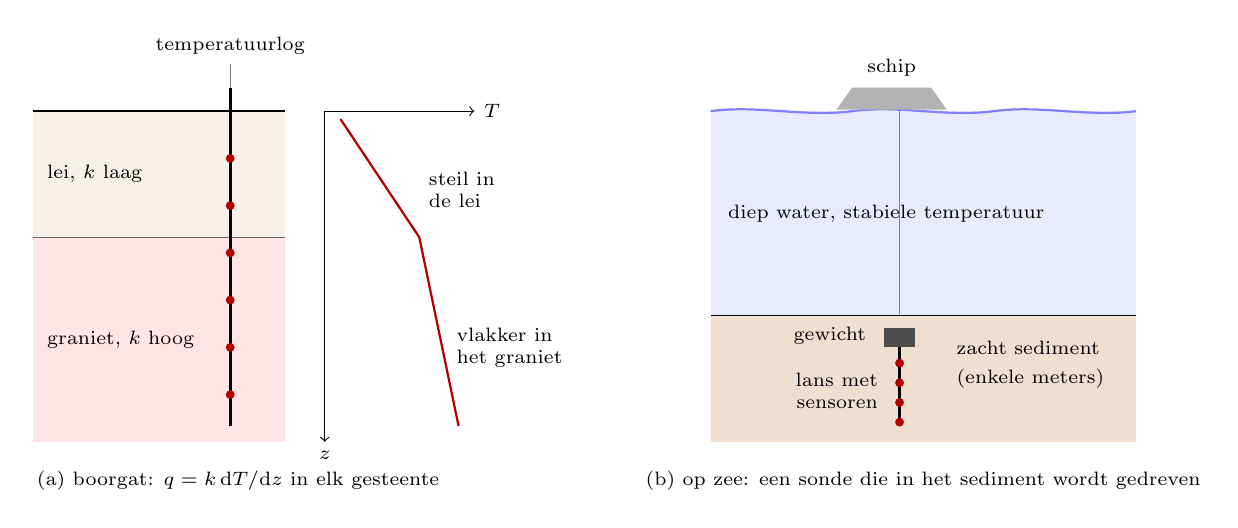
\begin{tikzpicture}[font=\scriptsize, x=1cm, y=1cm]
% --- left: borehole on land ---
\fill[brown!12] (0,0) rectangle (3.2,-1.6);
\fill[red!10] (0,-1.6) rectangle (3.2,-4.2);
\draw[thick] (0,0) -- (3.2,0);
\node[anchor=west] at (0.05,-0.8) {lei, $k$ laag};
\node[anchor=west] at (0.05,-2.9) {graniet, $k$ hoog};
\draw[black!60] (0,-1.6) -- (3.2,-1.6);
\draw[very thick] (2.5,0.3) -- (2.5,-4.0);
\draw[gray] (2.5,0.6) -- (2.5,0.3);
\foreach \y in {-0.6,-1.2,-1.8,-2.4,-3.0,-3.6} {\fill[red!70!black] (2.5,\y) circle (1.6pt);}
\node[anchor=south] at (2.5,0.6) {temperatuurlog};
% inset T(z)
\draw[->] (3.7,0) -- (5.6,0) node[right] {$T$};
\draw[->] (3.7,0) -- (3.7,-4.2) node[below] {$z$};
\draw[thick, red!70!black] (3.9,-0.1) -- (4.9,-1.6) -- (5.4,-4.0);
\node[anchor=west, align=left] at (4.9,-1.0) {steil in\\de lei};
\node[anchor=west, align=left] at (5.25,-3.0) {vlakker in\\het graniet};
\node[anchor=north] at (2.6,-4.45) {(a) boorgat: $q = k\,\mathrm dT/\mathrm dz$ in elk gesteente};
% --- right: probe at sea ---
\begin{scope}[xshift=8.6cm]
\fill[blue!8] (0,0) rectangle (5.4,-2.6);
\draw[blue!50, thick] (0,0) .. controls (0.6,0.08) and (1.2,-0.08) .. (1.8,0)
  .. controls (2.4,0.08) and (3.0,-0.08) .. (3.6,0) .. controls (4.2,0.08) and (4.8,-0.08) .. (5.4,0);
\fill[gray!60] (1.6,0.02) -- (3.0,0.02) -- (2.8,0.3) -- (1.8,0.3) -- cycle;
\node[anchor=south] at (2.3,0.32) {schip};
\draw[gray] (2.4,0.02) -- (2.4,-2.75);
\fill[brown!25] (0,-2.6) rectangle (5.4,-4.2);
\draw (0,-2.6) -- (5.4,-2.6);
\node[anchor=west] at (3.0,-3.0) {zacht sediment};
\node[anchor=west] at (3.0,-3.4) {(enkele meters)};
\fill[black!70] (2.2,-2.75) rectangle (2.6,-3.0);
\draw[very thick] (2.4,-3.0) -- (2.4,-4.0);
\foreach \y in {-3.2,-3.45,-3.7,-3.95} {\fill[red!70!black] (2.4,\y) circle (1.6pt);}
\node[anchor=east, align=right] at (2.1,-2.85) {gewicht};
\node[anchor=east, align=right] at (2.25,-3.55) {lans met\\sensoren};
\node[anchor=west] at (0.1,-1.3) {diep water, stabiele temperatuur};
\node[anchor=north] at (2.7,-4.45) {(b) op zee: een sonde die in het sediment wordt gedreven};
\end{scope}
\end{tikzpicture}

\par\smallskip{\small Het meten van de \omterm{def:b1:heat-budget:heat-flow}{warmtestroom} (schematisch, niet op schaal). (a) Op het land wordt de temperatuur in een boorgat gelogd zodra die weer in evenwicht is, en de geleidbaarheid van elk gesteente wordt op kernen gemeten: de gradiënt is steiler waar de geleidbaarheid lager is, en de \omterm{def:b1:heat-budget:heat-flow}{warmtestroom}, hun product, is overal gelijk. (b) Op zee wordt een lans met sensoren enkele meters in het sediment van de oceaanbodem gedreven.}
\label{fig:b1:heat-budget:measure}
\end{omfigure}

\begin{inthefield}[Warmtestroom op zee]
\begin{minipage}[t]{0.55\linewidth}\vspace{0pt}
Op een onderzoeksschip hangt de warmtestroomsonde als een zware lans aan de achterste kraan. Zij wordt aan de kabel van het schip tot net boven de zeebodem neergelaten en dan losgelaten: het gewicht drijft haar in het sediment, en de bemanning wacht op dek tot de sensoren op de temperatuur van de modder zijn ingesteld, haalt haar dan op en verplaatst het schip naar het volgende station, een klein stukje verder. Een rij van zulke stations dwars over een flank van een rug geeft de afname van de \omterm{def:b1:heat-budget:heat-flow}{warmtestroom} met de leeftijd van de bodem, en de spreiding tussen naburige stations toont waar water door de \omterm{def:b1:layered-earth:layers}{korst} eronder stroomt.
\end{minipage}\hfill
\begin{minipage}[t]{0.42\linewidth}\vspace{0pt}
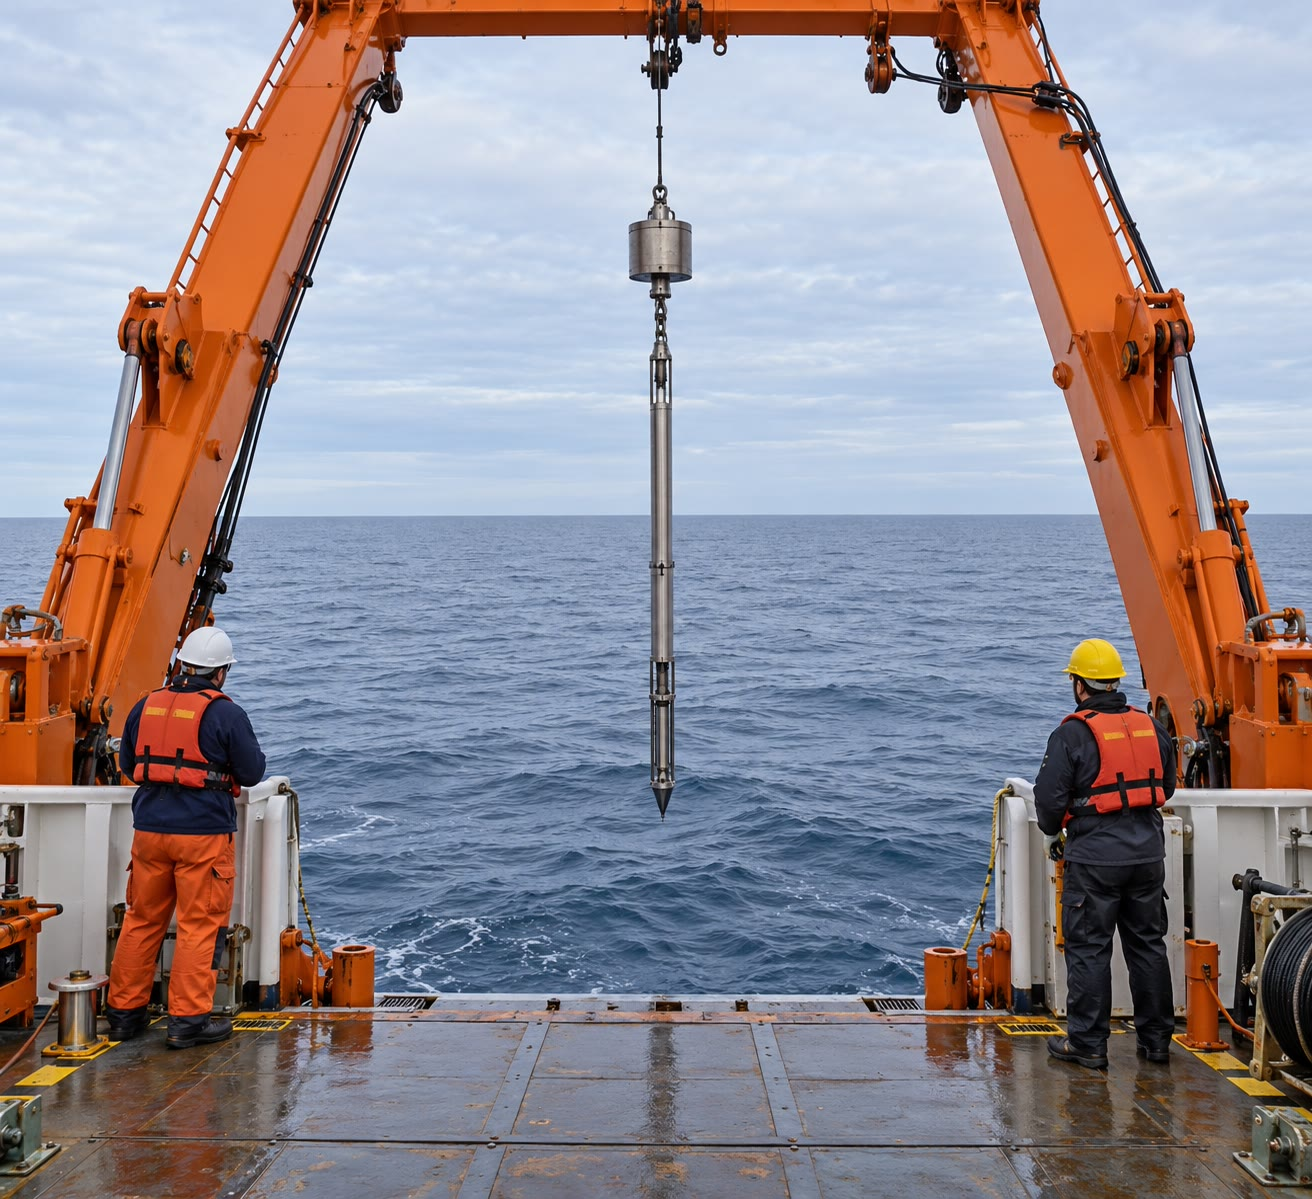
\includegraphics[width=\linewidth]{images/book3/ai/b1-heatflow-probe.jpg}

{\scriptsize Een warmtestroomsonde die aan de achterste kraan van een onderzoeksschip hangt
(door AI gegenereerde illustratie).}
\end{minipage}
\end{inthefield}

\section{De stationaire conductieve geotherm}

\begin{definition}[Geotherm]\label{def:b1:heat-budget:geotherm}
De \emph{geotherm}\index{geotherm} onder een punt van het oppervlak is de temperatuur als functie van de diepte daar, $T(z)$. Het is een stationaire conductieve geotherm wanneer zij niet met de tijd verandert en warmte er uitsluitend door geleiding langs wordt getransporteerd.
\end{definition}

Binnen de \omterm{def:b1:layered-earth:lithosphere}{lithosfeer}, ver van actieve vulkanen en van watercirculatie, wordt de warmte door geleiding vervoerd, en op een schaal van miljoenen jaren is de \omterm{def:b1:heat-budget:geotherm}{geotherm} stationair. Haar vorm volgt dan uit een energiebalans.

\begin{theorem}[Stationaire geleiding met warmteproductie]\label{thm:b1:heat-budget:balance}
Langs een stationaire conductieve \omterm{def:b1:heat-budget:geotherm}{geotherm}, in een medium met uniforme geleidbaarheid $k$, met warmteproductie $A(z)$ en zonder horizontale \omterm{def:b1:heat-budget:heat-flow}{warmtestroom},
\[
  \frac{\mathrm dq}{\mathrm dz} = -A(z), \qquad\text{dat is}\qquad
  k\,\frac{\mathrm d^2T}{\mathrm dz^2} = -A(z).
\]
\end{theorem}

\begin{proof}
Beschouw een horizontale plak met oppervlakte $S$ tussen de dieptes $z$ en $z +
\mathrm dz$. Warmte komt binnen via haar onderkant met een snelheid $q(z + \mathrm dz)\,S$, verlaat haar bovenkant met een snelheid $q(z)\,S$, en wordt van binnen geproduceerd met een snelheid $A(z)\,S\,\mathrm dz$. In een stationaire toestand wordt geen warmte opgeslagen, dus $q(z)\,S = q(z + \mathrm dz)\,S + A(z)\,S\,\mathrm dz$, wat $\mathrm dq/\mathrm dz = -A$ geeft. Volgens de wet van Fourier is $q = k\,\mathrm dT/\mathrm dz$, en met $k$ uniform is $k\,T'' = -A$.
\end{proof}

Van het oppervlak naar beneden gelezen neemt de \omterm{def:b1:heat-budget:heat-flow}{warmtestroom} met de diepte af met de warmte die boven elk niveau wordt geproduceerd: wat het oppervlak bereikt is de warmte die van onder komt plus alle warmte die onderweg is geproduceerd. Twee verdelingen van $A$ geven gesloten vormen.

\begin{proposition}[Een uniforme radiogene laag]\label{prop:b1:heat-budget:uniform}
Laat de warmteproductie $A$ zijn van het oppervlak tot de diepte $h$ en nul daaronder, het oppervlak op temperatuur $T_0$, en de \omterm{def:b1:heat-budget:heat-flow}{warmtestroom} aan het oppervlak $q_0$. Dan geldt voor $0 \le z \le h$
\[
  q(z) = q_0 - A z, \qquad T(z) = T_0 + \frac{q_0 z}{k} - \frac{A z^2}{2k},
\]
en onder $h$ is de \omterm{def:b1:heat-budget:heat-flow}{warmtestroom} uniform, $q_m = q_0 - A h$, en is de \omterm{def:b1:heat-budget:geotherm}{geotherm} een rechte lijn met helling $q_m/k$.
\end{proposition}

\begin{proof}
Integreer $\mathrm dq/\mathrm dz = -A$ vanaf $0$ met $q(0) = q_0$: $q = q_0 -
Az$. Dan is $\mathrm dT/\mathrm dz = (q_0 - Az)/k$; integreren met $T(0) = T_0$
geeft de parabool. Onder $h$ is $\mathrm dq/\mathrm dz = 0$ en behoudt $q$ haar
waarde op $h$.
\end{proof}

\begin{theorem}[Exponentiële warmteproductie en de lineaire warmtestroomrelatie]
\label{thm:b1:heat-budget:exponential}
Laat de warmteproductie met de diepte afnemen als $A(z) = A_0 e^{-z/D}$, de \omterm{def:b1:heat-budget:heat-flow}{warmtestroom} op grote diepte naar $q_m$ naderen, en het oppervlak op $T_0$ liggen. Dan
\[
  q(z) = q_m + A_0 D\,e^{-z/D}, \qquad
  T(z) = T_0 + \frac{q_m z}{k} + \frac{A_0 D^2}{k}\bigl(1 - e^{-z/D}\bigr),
\]
en de \omterm{def:b1:heat-budget:heat-flow}{warmtestroom} aan het oppervlak is
\[
  q_0 = q_m + A_0 D .
\]
\end{theorem}

\begin{proof}
Uit \cref{thm:b1:heat-budget:balance} volgt $\mathrm dq/\mathrm dz =
-A_0e^{-z/D}$, dus $q(z) = A_0 D e^{-z/D} + C$; voor $z \to \infty$ geldt $q \to C$,
dus $C = q_m$. Bij $z = 0$ is $q_0 = q_m + A_0 D$. Dan is $\mathrm dT/\mathrm dz =
q/k = q_m/k + (A_0D/k)\,e^{-z/D}$, en integreren vanaf $0$ met $T(0) = T_0$ geeft
$T = T_0 + q_m z/k + (A_0 D^2/k)(1 - e^{-z/D})$.
\end{proof}

De laatste regel is een voorspelling die aan het oppervlak kan worden getoetst. Graniet-plutons in één regio delen dezelfde diepe \omterm{def:b1:heat-budget:heat-flow}{warmtestroom} $q_m$ en, als zij alleen verschillen in hun rijkdom aan uranium, thorium en kalium, dezelfde schaal $D$; dan moet de \omterm{def:b1:heat-budget:heat-flow}{warmtestroom} die boven elke pluton wordt gemeten een lineaire functie zijn van de warmteproductie die op haar gesteenten is gemeten, met helling $D$ (een lengte) en snijpunt $q_m$, de gereduceerde \omterm{def:b1:heat-budget:heat-flow}{warmtestroom} die van onderen komt, onder de radiogene laag. Francis Birch zag zo'n lijn voor het eerst, gerapporteerd in 1968, en in hetzelfde jaar werden drie provincies gedefinieerd aan de hand van hun lijnen:
\begin{center}
\small
% ledger: roy:provinces, roy:linear-relation
\begin{tabular}{lcc}
\hline
provincie & snijpunt $q_m$ (\unit{mW.m^{-2}}) & helling $D$ (\unit{km}) \\
\hline
oostelijke Verenigde Staten & 33 & 7.5 \\
Basin and Range-provincie & 59 & 9.4 \\
Sierra Nevada & 17 & 10 \\
\hline
\end{tabular}
\end{center}
De snijpunten, gepubliceerd als 0.8, 1.4 en $0.4\times\qty{e-6}{cal.cm^{-2}.s^{-1}}$, worden omgerekend met $\qty{1}{\micro cal.cm^{-2}.s^{-1}} = \qty{41.84}{mW.m^{-2}}$ (\cref{exo:b1:heat-budget:4}). De hellingen variëren weinig, van 7 tot \qty{10}{km}; de gereduceerde \omterm{def:b1:heat-budget:heat-flow}{warmtestroom} varieert veel, en kaarten ervan tonen waar de \omterm{def:b1:layered-earth:layers}{mantel} eronder heet is, zoals onder de uitgerekte \omterm{def:b1:layered-earth:layers}{korst} van de Basin and Range. De uniforme laag van \cref{prop:b1:heat-budget:uniform} geeft ook een rechte lijn, met helling $h$: beide modellen passen op de gegevens, maar alleen het exponentiële model blijft een rechte lijn met dezelfde helling wanneer de plutons tot verschillende diepten zijn geërodeerd (\cref{exo:b1:heat-budget:10}), en daarom heeft het de voorkeur.

\begin{omfigure}
\begin{tikzpicture}
\begin{axis}[omdepth, width=0.82\linewidth, height=8.6cm, xmin=0, xmax=1800, ymin=0, ymax=250, axis x line=top, axis y line=left, axis line style={-}, clip=true,
  xlabel={temperatuur (\unit{\degreeCelsius})}, ylabel={diepte (km)},
  tick label style={font=\scriptsize}, label style={font=\small},
  legend style={font=\scriptsize, at={(0.02,0.02)}, anchor=south west, draw=none, fill=white, fill opacity=0.85, text opacity=1},
  legend cell align=left]
\addplot[very thick, black!45] table[x=T, y=depth] {figdata/out/bachelor-1-geotherms-adiabat.dat};
\addlegendentry{mantel-adiabaat}
\addplot[very thick, red!75!black] table[x=T45, y=depth] {figdata/out/bachelor-1-geotherms-continental.dat};
\addlegendentry{$q_0 = \qty{70}{mW.m^{-2}}$}
\addplot[very thick, orange!80!black] table[x=T30, y=depth] {figdata/out/bachelor-1-geotherms-continental.dat};
\addlegendentry{$q_0 = \qty{55}{mW.m^{-2}}$}
\addplot[very thick, green!45!black] table[x=T15, y=depth] {figdata/out/bachelor-1-geotherms-continental.dat};
\addlegendentry{$q_0 = \qty{40}{mW.m^{-2}}$}
\addplot[thick, blue!70!black, densely dashdotted] table[x=T, y=depth] {figdata/out/bachelor-1-geotherms-oceanic.dat};
\addlegendentry{oceaanbodem van \qty{60}{Myr} oud}
\addplot[thin, dashed, red!75!black, forget plot] table[x=Tc45, y=depth] {figdata/out/bachelor-1-geotherms-continental.dat};
\addplot[thin, dashed, orange!80!black, forget plot] table[x=Tc30, y=depth] {figdata/out/bachelor-1-geotherms-continental.dat};
\addplot[thin, dashed, green!45!black, forget plot] table[x=Tc15, y=depth] {figdata/out/bachelor-1-geotherms-continental.dat};
\draw[densely dotted, black!60] (axis cs:0,35) -- (axis cs:1800,35);
\node[font=\scriptsize, anchor=south east] at (axis cs:1790,35) {Moho, \qty{35}{km}};
\fill (axis cs:1384.0,70.8) circle (1.6pt);
\fill (axis cs:1403.2,107.8) circle (1.6pt);
\fill (axis cs:1459.7,224.9) circle (1.6pt);
\node[font=\scriptsize, anchor=west] at (axis cs:1420,66) {\qty{71}{km}};
\node[font=\scriptsize, anchor=west] at (axis cs:1440,104) {\qty{108}{km}};
\node[font=\scriptsize, anchor=west] at (axis cs:1495,222) {\qty{225}{km}};
\end{axis}
\end{tikzpicture}

\par\smallskip{\small Stationaire conductieve \omterm{def:b1:heat-budget:geotherm}{geotherms} van een continent met warmteproductie $A_0 = \qty{2.5}{\micro W.m^{-3}}$ die over $D = \qty{10}{km}$ afneemt, $k = \qty{2.5}{W.m^{-1}.K^{-1}}$, voor drie oppervlaktewarmtestromen (gereduceerde \omterm{def:b1:heat-budget:heat-flow}{warmtestroom} 15, 30 en \qty{45}{mW.m^{-2}}). Elke volgt zijn conductieve kromme (gestreept na dat punt) tot de \omterm{def:b1:heat-budget:adiabat}{mantel-adiabaat}, die zij bij het stipje ontmoet: de basis van de \omterm{def:b1:heat-budget:boundary-layer}{thermische lithosfeer}. De \omterm{def:b1:heat-budget:geotherm}{geotherm} van de oceaanbodem is die van een halfruimte die gedurende \qty{60}{Myr} is afgekoeld. Uniforme geleidbaarheid is een vereenvoudiging.}
\label{fig:b1:heat-budget:geotherms}
\end{omfigure}

\begin{method}[De temperatuur op diepte onder een pluton]\label{met:b1:heat-budget:moho}
\begin{enumerate}
  \item Meet de oppervlaktewarmtestroom $q_0$ boven de pluton (boormethode) en haar warmteproductie $A_0$ uit haar gehalte aan U, Th en K.
  \item Bereken uit de rechte lijn van de provincie, of met een waarde van $D$ van ongeveer \qty{10}{km}, $q_m = q_0 - A_0 D$.
  \item Pas \cref{thm:b1:heat-budget:exponential} toe. Onder enkele malen $D$ is $e^{-z/D}$ verwaarloosbaar en is de \omterm{def:b1:heat-budget:geotherm}{geotherm} de rechte lijn $T_0 + A_0D^2/k + q_m z/k$: de radiogene laag heeft elke diepe temperatuur met $A_0D^2/k$ verhoogd.
\end{enumerate}
\end{method}

In de figuur loopt de temperatuur bij de \omterm{def:b1:layered-earth:discontinuity}{Moho} van ongeveer \qty{320}{\degreeCelsius} voor de laagste \omterm{def:b1:heat-budget:heat-flow}{warmtestroom} tot meer dan \qty{700}{\degreeCelsius} voor de hoogste: de \omterm{def:b1:heat-budget:heat-flow}{warmtestroom} aan het oppervlak geeft een direct beeld van de temperatuur van de diepe \omterm{def:b1:layered-earth:layers}{korst}, die haar sterkte bepaalt (\cref{ch:b1:stress-strain-rheology}).

\section{Geleiding tegen convectie}

Geleiding is traag. Hoe traag volgt uit de warmtevergelijking, die de natuurkundeboeken afleiden uit de wet van Fourier en de balans van \cref{thm:b1:heat-budget:balance} met opslag erbij: in één dimensie, zonder warmteproductie,
$\partial T/\partial t = \kappa\,\partial^2 T/\partial z^2$.

\begin{proposition}[De conductieve tijdschaal]\label{prop:b1:heat-budget:timescale}
Een temperatuurverandering die aan een grens van een geleidend lichaam wordt opgelegd, verspreidt zich over een afstand $L$ in een tijd van de orde van
\[
  \tau = \frac{L^2}{\kappa} .
\]
\end{proposition}

\begin{proof}
Schrijf $z = L z^*$, $t = \tau t^*$, met $z^*$ en $t^*$ dimensieloos. De warmtevergelijking wordt $\partial T/\partial t^* = (\kappa\tau/L^2)\,\partial^2
T/\partial z^{*2}$. Haar oplossingen variëren op de schaal $z^* \sim 1$ wanneer $t^* \sim 1$ alleen als de coëfficiënt van orde één is, dat wil zeggen als $\tau \sim L^2/\kappa$.
\end{proof}

Gesteenten hebben $\kappa \approx \qty{e-6}{m^2.s^{-1}}$. De dagelijkse temperatuurcyclus reikt enkele tientallen centimeters in de grond, de jaarlijkse enkele meters, en de opwarming sinds de laatste ijstijd een kilometer of zo. Over een \omterm{def:b1:layered-earth:lithosphere}{lithosfeer} van \qty{100}{km} dik is $\tau = \qty{e16}{s}$, ongeveer \qty{300}{Myr}. Over de \omterm{def:b1:layered-earth:layers}{mantel}, \qty{2900}{km} dik, is $\tau = \qty{8.4e18}{s}$, of \qty{270}{Gyr}: zestig keer de leeftijd van de aarde, \qty{4.54}{Gyr}. % ledger: england:kelvin, usgs:age-earth
Geleiding alleen zou de warmte van de diepe \omterm{def:b1:layered-earth:layers}{mantel} nooit in de buurt van het oppervlak hebben kunnen brengen. De \omterm{def:b1:layered-earth:layers}{mantel} convecteert, en in haar binnenste wordt de warmte vervoerd door de beweging van het gesteente zelf, met de snelheden van de platen, centimeters per jaar. % ledger: usgs:san-andreas

\begin{definition}[Mantel-adiabaat]\label{def:b1:heat-budget:adiabat}
De \emph{mantel-adiabaat}\index{mantel-adiabaat} is de \omterm{def:b1:heat-budget:geotherm}{geotherm} van het goed gemengde binnenste van de convecterende \omterm{def:b1:layered-earth:layers}{mantel}: de temperatuur die mantelgesteente aanneemt wanneer het snel genoeg stijgt of zinkt om geen warmte met zijn omgeving uit te wisselen, afkoelend bij het stijgen door uitzetting en opwarmend bij het zinken door samendrukking.
\end{definition}

Thermodynamica geeft de gradiënt ervan, $\mathrm dT/\mathrm dz = \alpha g T/c_p$, met $\alpha$ de thermische uitzettingscoëfficiënt en $c_p$ de soortelijke warmte (natuurkunde, hier aangenomen). Hij is klein. Een recente evaluatie uit de mineraalfysica geeft \qty{0.54}{K.km^{-1}} op \qty{50}{km} diepte, dalend tot \qty{0.36}{K.km^{-1}} op \qty{410}{km}, daarna 0.41 tot \qty{0.23}{K.km^{-1}} door de onderste \omterm{def:b1:layered-earth:layers}{mantel}, met \qty{1646}{K} op \qty{50}{km} en \qty{2587}{K} op \qty{2800}{km}.
% ledger: katsura:adiabat
Geëxtrapoleerd tot het oppervlak geeft de adiabaat de potentiële temperatuur van de \omterm{def:b1:layered-earth:layers}{mantel}, \qty{1619}{K} of ongeveer \qty{1350}{\degreeCelsius}: de temperatuur die de \omterm{def:b1:layered-earth:layers}{mantel} zou hebben als zij zonder warmte-uitwisseling naar het oppervlak werd gebracht. Het begrip potentiële temperatuur wordt, voor de atmosfeer en de oceaan, gedefinieerd in \cref{ch:b1:fluid-envelopes-structure}. Een temperatuur die met de diepte maar \qty{0.5}{K} per kilometer stijgt, terwijl de conductieve \omterm{def:b1:heat-budget:geotherm}{geotherm} nabij het oppervlak met \qty{25}{K} stijgt, is het kenmerk van convectie.

\begin{history}[John Perry en de afkoelende aarde]
In 1862--1863 berekende William Thomson, later Lord Kelvin, de leeftijd van de aarde uit haar afkoeling. Hij behandelde haar als een vaste stof die door geleiding was afgekoeld vanaf een uniforme temperatuur van ongeveer \qty{3900}{\degreeCelsius}; met de gemiddelde gradiënt die hij toen uit de metingen van zijn tijd koos, ongeveer \qty{36}{K.km^{-1}}, en een diffusiviteit van \qty{1.2e-6}{m^2.s^{-1}}, bedroeg de tijd om de huidige gradiënt te bereiken ongeveer \qty{96}{Myr}, tussen grenzen van 24 en \qty{400}{Myr} (\cref{exo:b1:heat-budget:9}). Geologen vonden dit veel te kort. In 1895, een jaar voordat radioactiviteit werd ontdekt, wees zijn voormalige assistent John Perry op een aanname: als het binnenste gedeeltelijk vloeibaar was en convecteerde, zou het warmte dragen alsof het een enorme geleidbaarheid had, en zou het hele binnenste, niet een dunne buitenschil, de \omterm{def:b1:heat-budget:heat-flow}{warmtestroom} aan het oppervlak voeden. Zijn argument werd genegeerd en vergeten; de mantelconvectie, lang daarna vastgesteld, bewees hem gelijk: de diepe \omterm{def:b1:layered-earth:layers}{mantel} koelt af door convectie, en dat is de \omterm{def:b1:heat-budget:secular-cooling}{seculiere afkoeling} van de balans. % ledger: england:kelvin, england:perry
\end{history}

\begin{proposition}[Perry's goed doorgeroerde aarde]\label{prop:b1:heat-budget:perry}
Laat een bol met straal $R$ een goed doorgeroerd binnenste hebben op de uniforme temperatuur $T_i(t)$, met warmtecapaciteit $\rho c$ per volume-eenheid, onder een geleidend deksel met dikte $L \ll R$ en geleidbaarheid $k$ waarvan het oppervlak op $\qty{0}{\degreeCelsius}$ ligt, en laat er geen warmteproductie zijn. Dan geldt
\[
  T_i(t) = T_i(0)\,e^{-t/\tau_P}, \qquad \tau_P = \frac{RL}{3\kappa},
\]
en de oppervlaktewarmtestroom $kT_i/L$ vervalt met dezelfde tijdconstante.
\end{proposition}

\begin{proof}
Omdat het deksel dun is, verkeert het in een stationaire toestand en draagt het de \omterm{def:b1:heat-budget:heat-flow}{warmtestroom} $q = kT_i/L$. Het binnenste verliest zijn warmte via het oppervlak $4\pi R^2$:
$\tfrac43\pi R^3\rho c\,\mathrm dT_i/\mathrm dt = -4\pi R^2 kT_i/L$, dat wil zeggen
$\mathrm dT_i/\mathrm dt = -3\kappa T_i/(RL)$ met $\kappa = k/(\rho c)$, waarvan de oplossing de exponentiële functie is met $\tau_P = RL/(3\kappa)$.
\end{proof}

Voor $R = \qty{6400}{km}$, $L = \qty{100}{km}$ en $\kappa =
\qty{e-6}{m^2.s^{-1}}$, $\tau_P = \qty{6.8}{Gyr}$: een convecterende aarde houdt miljarden jaren een hoge \omterm{def:b1:heat-budget:heat-flow}{warmtestroom}, waar de geleidende aarde van Kelvin haar in tientallen miljoenen jaren verloor (\cref{exo:b1:heat-budget:11}).

\section{De lithosfeer als thermische grenslaag}\label{sec:b1:heat-budget:boundary-layer}

\begin{definition}[Thermische grenslaag, thermische lithosfeer]\label{def:b1:heat-budget:boundary-layer}
In een convecterende vloeistof is een \emph{thermische grenslaag}\index{thermische grenslaag} een laag langs een grens waarheen warmte door geleiding gaat en waarin de temperatuur overgaat van die van de grens naar die van het goed gemengde binnenste. De \emph{thermische lithosfeer}\index{thermische lithosfeer} is de bovenste thermische grenslaag van de \omterm{def:b1:layered-earth:layers}{mantel}: de buitenste schil van de aarde van het oppervlak tot de diepte waar de conductieve \omterm{def:b1:heat-budget:geotherm}{geotherm} de \omterm{def:b1:heat-budget:adiabat}{mantel-adiabaat} ontmoet.
\end{definition}

De platen zijn de koude top van de convectie van de \omterm{def:b1:layered-earth:layers}{mantel}, haar bovenste grenslaag. Hun basis, waar de steile conductieve \omterm{def:b1:heat-budget:geotherm}{geotherm} buigt naar de zachte adiabaat, ligt op \qtyrange{70}{230}{km} in de figuur van de \omterm{def:b1:heat-budget:geotherm}{geotherms} voor continentale warmtestromen van 70 tot \qty{40}{mW.m^{-2}}, binnen het bereik dat de seismologie meet (\cref{ch:b1:layered-earth}): de \omterm{def:b1:layered-earth:lithosphere}{lithosfeer} die door haar sterkte is bepaald en de \omterm{def:b1:layered-earth:lithosphere}{lithosfeer} die door haar temperatuur is bepaald zijn ongeveer dezelfde schil, omdat sterkte van de temperatuur afhangt. Aan de onderkant van de \omterm{def:b1:layered-earth:layers}{mantel} is de D$''$-laag de onderste grenslaag, van onderen verwarmd door de kern.

Onder de oceanen ontstaat de grenslaag bij de rug, waar heet mantelgesteente naar het oppervlak stijgt, en zij wordt dikker naarmate de plaat zich verwijdert en afkoelt. De afkoeling van een halfruimte vanaf een uniforme temperatuur, door Fourier opgelost en door Kelvin voor de hele aarde gebruikt, beschrijft haar goed (\cref{ch:b1:rifts-ridges-margins}; de afleiding volgt in Boek 5): de isothermen verdiepen zich met de vierkantswortel van de leeftijd van de bodem (figuur hieronder), en de \omterm{def:b1:heat-budget:heat-flow}{warmtestroom} neemt af als
\[
  q(t) = \frac{C}{\sqrt t}, \qquad C \approx \qty{490}{mW.m^{-2}.Myr^{1/2}},
\]
de waarde die in de wereldwijde balans wordt gebruikt. % ledger: dd10:young-ocean
Op \qty{100}{Myr} is de halfruimte afgekoeld tot ongeveer \qty{130}{km} (\cref{exo:b1:heat-budget:12}). De echte plaat stopt eerder met verdikken: seismische golven die de Stille Oceaan doorkruisen worden het best gepast door een afkoelende plaat die naar een dikte van \qtyrange{85}{95}{km} neigt, de afvlakking van oude zeebodem die in \cref{ch:b1:rifts-ridges-margins} opnieuw aan bod komt.
% ledger: fischer:lithosphere

De warmtebalans, de \omterm{def:b1:heat-budget:heat-flow}{warmtestroom} en de thermische structuur van de platen komen samen in de volgende hoofdstukken: de afkoelende plaat zakt weg (\cref{ch:b1:rifts-ridges-margins}), en de koude \omterm{def:b1:layered-earth:lithosphere}{lithosfeer} die bij subductiezones zinkt is de neerwaartse stroming van de convectie waartoe zij behoort.

\begin{omfigure}
\begin{tikzpicture}
\begin{axis}[width=0.86\linewidth, height=5.6cm, xmin=0, xmax=100, ymin=0, ymax=170,
  y dir=reverse, axis x line=top, axis y line=left, axis line style={-}, clip=false,
  xlabel={leeftijd van de oceaanbodem (Myr), toenemend met de afstand tot de rug},
  ylabel={diepte (km)}, tick label style={font=\scriptsize}, label style={font=\small}]
\addplot[fill=blue!12, draw=none] table[x=age, y=z1200] {figdata/out/bachelor-1-geotherms-isotherms.dat} \closedcycle;
\addplot[thick, blue!30!black] table[x=age, y=z400] {figdata/out/bachelor-1-geotherms-isotherms.dat};
\addplot[thick, blue!50!red] table[x=age, y=z800] {figdata/out/bachelor-1-geotherms-isotherms.dat};
\addplot[very thick, red!75!black] table[x=age, y=z1200] {figdata/out/bachelor-1-geotherms-isotherms.dat};
\node[font=\scriptsize, anchor=south, fill=blue!12, inner sep=1pt] at (axis cs:80,24) {\qty{400}{\degreeCelsius}};
\node[font=\scriptsize, anchor=south, fill=blue!12, inner sep=1pt] at (axis cs:80,55) {\qty{800}{\degreeCelsius}};
\node[font=\scriptsize, anchor=south, fill=blue!12, inner sep=1pt] at (axis cs:80,108) {\qty{1200}{\degreeCelsius}};
\node[font=\small] at (axis cs:60,72) {thermische lithosfeer};
\node[font=\small] at (axis cs:55,150) {convecterende mantel, ongeveer \qty{1350}{\degreeCelsius}};
\draw[->, thick, red!60!black] (axis cs:3,165) -- (axis cs:3,125);
\node[font=\scriptsize, anchor=west, red!60!black] at (axis cs:4,140) {opstijgend onder de rug};
\draw[->, thick, black!60] (axis cs:30,5) -- (axis cs:70,5);
\node[font=\scriptsize, anchor=west] at (axis cs:70,5) {plaatbeweging};
\end{axis}
\end{tikzpicture}

\par\smallskip{\small Isothermen in een afkoelende oceanische plaat: een halfruimte die aanvankelijk op \qty{1350}{\degreeCelsius} is, afgekoeld vanaf haar oppervlak, met $\kappa = \qty{e-6}{m^2.s^{-1}}$. Elke isotherm verdiept zich met de vierkantswortel van de leeftijd; de gearceerde laag boven de \qty{1200}{\degreeCelsius}-isotherm is de \omterm{def:b1:heat-budget:boundary-layer}{thermische lithosfeer}. Pijlen zijn schematisch.}
\label{fig:b1:heat-budget:isotherms}
\end{omfigure}

\section{Oefeningen}

\begin{exercise}[$\star$]\label{exo:b1:heat-budget:1}
Een boorgat in graniet met geleidbaarheid \qty{2.5}{W.m^{-1}.K^{-1}} toont een stationaire gradiënt van \qty{22}{K.km^{-1}}. Bereken de \omterm{def:b1:heat-budget:heat-flow}{warmtestroom} en het vermogen dat ter plaatse door één vierkante kilometer oppervlak gaat.
% ledger: delaney:conductivity
\end{exercise}

\begin{exercise}[$\star$]\label{exo:b1:heat-budget:2}
Bereken uit de oppervlakten en de gemiddelde warmtestromen van de continenten (\qty{2.073e14}{m^2}, \qty{70.9}{mW.m^{-2}}) en de oceanen (\qty{3.028e14}{m^2}, \qty{105.4}{mW.m^{-2}}) het warmteverlies van elk, het totaal en de gemiddelde \omterm{def:b1:heat-budget:heat-flow}{warmtestroom} over het oppervlak van de aarde (\qty{5.101e14}{m^2}). Welk deel van de \qty{173000}{TW} die van de zon wordt ontvangen, is dat?
% ledger: dd10:split, nasa:solar-mean
\end{exercise}

\begin{exercise}[$\star$]\label{exo:b1:heat-budget:3}
Bereken uit de tabel van de vier isotopen de warmte die per kilogram natuurlijk uranium vrijkomt (\qty{99.274}{\percent} \ce{^{238}U} en \qty{0.720}{\percent} \ce{^{235}U} van de atomen; hun massa's verschillen met ongeveer \qty{1}{\percent}, dus neem deze als massafracties) en per kilogram natuurlijk kalium, waarvan \ce{^{40}K} \qty{0.0117}{\percent} van de atomen uitmaakt (neem de massa van een \ce{^{40}K}-atoom $39.96/39.10$ keer de gemiddelde massa van een kaliumatoom).
% ledger: dye:isotope-heat, iaea:isotopes
\end{exercise}

\begin{exercise}[$\star$]\label{exo:b1:heat-budget:4}
Reken de snijpunten van de drie provincies, 0.8, 1.4 en
$0.4\times\qty{e-6}{cal.cm^{-2}.s^{-1}}$, om in \unit{mW.m^{-2}}
($\qty{1}{cal} = \qty{4.184}{J}$). Voorspel de oppervlaktewarmtestroom boven een graniet met een warmteproductie van \qty{3.0}{\micro W.m^{-3}} in elke provincie.
% ledger: roy:provinces
\end{exercise}

\begin{exercise}[$\star\star$]\label{exo:b1:heat-budget:5}
Een \omterm{def:b1:layered-earth:layers}{korst} heeft een uniforme warmteproductie van \qty{2.0}{\micro W.m^{-3}} in haar bovenste \qty{10}{km} en geen daaronder, een geleidbaarheid van \qty{2.5}{W.m^{-1}.K^{-1}}, een oppervlaktewarmtestroom van \qty{60}{mW.m^{-2}} en een oppervlaktetemperatuur van \qty{10}{\degreeCelsius}. Bereken de temperatuur op \qty{10}{km}, de \omterm{def:b1:heat-budget:heat-flow}{warmtestroom} onder de radiogene laag, en de temperatuur bij de \omterm{def:b1:layered-earth:discontinuity}{Moho}, \qty{35}{km} diep.
\end{exercise}

\begin{exercise}[$\star\star$]\label{exo:b1:heat-budget:6}
Een boorgat doorkruist \qty{300}{m} schalie ($k = \qty{1.5}{W.m^{-1}.K^{-1}}$), daarna graniet ($k = \qty{3.0}{W.m^{-1}.K^{-1}}$). De evenwichtstemperaturen zijn \qty{12.0}{\degreeCelsius} aan het oppervlak, \qty{24.0}{\degreeCelsius} op \qty{300}{m} en \qty{34.0}{\degreeCelsius} op \qty{800}{m}. Bereken de gradiënt en de \omterm{def:b1:heat-budget:heat-flow}{warmtestroom} in elk gesteente, de thermische weerstand op \qty{300}{m} en op \qty{800}{m}, en de helling van het Bullard-diagram. Is de \omterm{def:b1:heat-budget:heat-flow}{warmtestroom} constant?
\end{exercise}

\begin{exercise}[$\star\star$]\label{exo:b1:heat-budget:7}
Bereken met $\kappa = \qty{e-6}{m^2.s^{-1}}$ de conductieve tijdschaal voor $L = \qty{1}{m}$, \qty{10}{m}, \qty{100}{km} en \qty{2900}{km}, elk in een geschikte eenheid. Welke cycli van de oppervlaktetemperatuur zijn nog \qty{10}{m} onder de grond voelbaar? Vergelijk de laatste tijd met de leeftijd van de aarde.
% ledger: england:kelvin, usgs:age-earth
\end{exercise}

\begin{exercise}[$\star\star$]\label{exo:b1:heat-budget:8}
De \omterm{def:b1:heat-budget:adiabat}{mantel-adiabaat} ligt op \qty{1646}{K} op \qty{50}{km} diepte, met daar een gradiënt van \qty{0.54}{K.km^{-1}}, dalend tot \qty{0.36}{K.km^{-1}} op \qty{410}{km}. (a) Extrapoleer haar tot het oppervlak met de gradiënt op \qty{50}{km}, en geef de potentiële temperatuur in kelvin en in graden Celsius. (b) Schat de temperatuur op \qty{410}{km} met het gemiddelde van de twee gradiënten, en vergelijk met de gepubliceerde \qty{1799}{K} net boven de discontinuïteit.
% ledger: katsura:adiabat
\end{exercise}

\begin{exercise}[$\star\star$]\label{exo:b1:heat-budget:9}
Een halfruimte die vanaf de uniforme temperatuur $T_0$ is afgekoeld, met haar oppervlak op $\qty{0}{\degreeCelsius}$ gehouden, heeft na een tijd $t$ de oppervlaktegradiënt $G =
T_0/\sqrt{\pi\kappa t}$ (aangenomen). (a) Druk $t$ uit in termen van $G$. (b) Met de waarden van Kelvin, $T_0 = \qty{3900}{\degreeCelsius}$, $\kappa =
\qty{1.2e-6}{m^2.s^{-1}}$ en $G = 1/50$ graad Fahrenheit per voet, bereken $G$ in \unit{K.km^{-1}} en de leeftijd. (c) Herhaal het met $T_0 =
\qty{1300}{\degreeCelsius}$, $\kappa = \qty{e-6}{m^2.s^{-1}}$ en $G =
\qty{36}{K.km^{-1}}$.
% ledger: england:kelvin
\end{exercise}

\begin{exercise}[$\star\star\star$]\label{exo:b1:heat-budget:10}
Een provincie wordt geërodeerd: een dikte $e$ wordt van de bovenkant van elke pluton verwijderd, terwijl de diepe \omterm{def:b1:heat-budget:heat-flow}{warmtestroom} $q_m$ onveranderd blijft. (a) Laat in het exponentiële model zien dat de nieuwe oppervlaktewarmteproductie en -warmtestroom, $A_0'$ en $q_0'$, nog steeds voldoen aan $q_0' = q_m + A_0'D$. (b) Laat in het uniforme-lagenmodel met dikte $h$ zien dat een pluton die met $e$ is geërodeerd op een lijn met helling $h - e$ ligt. (c) Plutons van één provincie zijn met verschillende hoeveelheden geërodeerd. Welk model voorspelt dat zij nog steeds op één lijn liggen?
\end{exercise}

\begin{exercise}[$\star\star\star$]\label{exo:b1:heat-budget:11}
In Perry's model (\cref{prop:b1:heat-budget:perry}) neem $R = \qty{6400}{km}$, $\kappa = \qty{e-6}{m^2.s^{-1}}$, $k = \qty{3}{W.m^{-1}.K^{-1}}$ en een begininterne temperatuur van \qty{1300}{\degreeCelsius}. (a) Bereken $\tau_P$ voor deksels van 50 en \qty{100}{km}. (b) Bereken voor het deksel van \qty{50}{km} de oppervlaktewarmtestroom bij het begin en na \qty{2}{Gyr}. (c) De geleidende halfruimte van Kelvin met dezelfde $k$ en $T_0$ heeft een oppervlaktewarmtestroom $kT_0/\sqrt{\pi\kappa t}$: bereken die na \qty{2}{Gyr} en vergelijk.
% ledger: england:kelvin, england:perry
\end{exercise}

\begin{exercise}[$\star\star\star$]\label{exo:b1:heat-budget:12}
De oppervlaktewarmtestroom van een afkoelende halfruimte is $q = k\,\Delta T/\sqrt{\pi\kappa t}$ (\cref{exo:b1:heat-budget:9}). (a) Met $k = \qty{3}{W.m^{-1}.K^{-1}}$, $\kappa =
\qty{e-6}{m^2.s^{-1}}$ en $\Delta T = \qty{1336}{K}$ (van de potentiële temperatuur tot een zeebodem van ongeveer \qty{10}{\degreeCelsius}), bereken de constante $C$ van $q = C/\sqrt t$, met $t$ in miljoenen jaren, en vergelijk haar met de \qty{490}{mW.m^{-2}.Myr^{1/2}} die aan de gegevens is gefit. (b) Met $C = 490$, geef de \omterm{def:b1:heat-budget:heat-flow}{warmtestroom} op 1, 10 en \qty{100}{Myr}. (c) De \qty{1200}{\degreeCelsius}-isotherm uit de figuur van de afkoelende isothermen ligt waar $z = 2\times1.163\sqrt{\kappa t}$; bereken haar diepte op \qty{100}{Myr}.
% ledger: dd10:young-ocean, katsura:adiabat, fischer:lithosphere
\end{exercise}

\section{Probleem: Hete gesteenten onder de plutons}

\begin{problem}[{Weekendprobleem --- warmtestroom en warmteproductie van vijf graniet-plutons, de lineaire
relatie, en de temperatuur van de diepe korst}]
\label{pb:b1:heat-budget:1}
% values: calc/ch10.py (invented province; element heats from the chapter's table)
% ledger: dye:isotope-heat, iaea:isotopes, dd10:split, roy:provinces
Vijf graniet-plutons van één provincie zijn geboord. In elk boorgat werd de \omterm{def:b1:comparative-planetology:equilibrium-temperature}{evenwichtstemperatuur} gelogd op \qty{100}{m} en op \qty{500}{m}, en de geleidbaarheid van het graniet werd op kernen gemeten; het gehalte aan uranium, thorium en kalium werd geanalyseerd op monsters van het oppervlak. Alle vijf granieten hebben een dichtheid van \qty{2650}{kg.m^{-3}}.
\begin{center}
\small
\begin{tabular}{cccccc}
\hline
pluton & $T$ op \qty{100}{m} (\unit{\degreeCelsius}) & $T$ op \qty{500}{m} (\unit{\degreeCelsius}) & $k$ (\unit{W.m^{-1}.K^{-1}}) & U, Th (ppm) & K (\unit{\percent}) \\
\hline
A & 13.1 & 19.2 & 2.9 & 2.0, 8 & 3.0 \\
B & 12.4 & 20.2 & 2.6 & 3.5, 14 & 3.5 \\
C & 13.6 & 21.4 & 3.1 & 5.0, 18 & 4.0 \\
D & 12.9 & 23.1 & 2.7 & 7.0, 25 & 4.2 \\
E & 14.2 & 25.5 & 3.0 & 10.0, 35 & 4.5 \\
\hline
\end{tabular}
\end{center}
Gebruik de warmteproducties van de elementen $\qty{9.85e-5}{W.kg^{-1}}$ (U), $\qty{2.63e-5}{W.kg^{-1}}$ (Th) en $\qty{3.40e-9}{W.kg^{-1}}$ (K). Neem onder de plutons $k = \qty{2.5}{W.m^{-1}.K^{-1}}$ voor de hele \omterm{def:b1:layered-earth:layers}{korst} en een oppervlaktetemperatuur van \qty{10}{\degreeCelsius}.

\medskip
\noindent\textbf{Deel I --- Warmtestroom.}
\begin{enumerate}
  \item Bereken de temperatuurgradiënt in elk boorgat.
  \item Waarom moeten de temperaturen weken of maanden na het boren worden gelogd, en waarom wordt de bovenste \qty{100}{m} weggelaten?
  \item Bereken de \omterm{def:b1:heat-budget:heat-flow}{warmtestroom} bij elke pluton.
  \item Vergelijk die met de gemiddelde continentale \omterm{def:b1:heat-budget:heat-flow}{warmtestroom}, \qty{70.9}{mW.m^{-2}}.
  \item De gradiënten van B en C zijn gelijk. Waarom zijn hun warmtestromen dat niet?
  \item De plutons liggen onder heuvels. Zou het reliëf de gemeten gradiënt onder een top verhogen of verlagen? (Denk aan de vorm van de isothermen.)
\end{enumerate}

\noindent\textbf{Deel II --- Warmteproductie en de lijn.}
\begin{enumerate}[resume]
  \item Bereken de warmteproductie door uranium in elke pluton.
  \item Idem voor thorium.
  \item Idem voor kalium.
  \item Tel ze op tot $A_0$ voor elke pluton. Welk element draagt het minst bij?
  \item Zet $q_0$ uit tegen $A_0$. Liggen de punten dicht bij een rechte lijn?
  \item Bereken de gemiddelden van $A_0$ en $q_0$, en de sommen
        $\sum (A_0 - \bar A_0)^2$ en $\sum (A_0 - \bar A_0)(q_0 - \bar q_0)$.
  \item Leid de kleinste-kwadratenlijn $q_0 = q_m + D A_0$ af: haar helling $D$ (in
        \unit{km}) en haar snijpunt $q_m$.
  \item Vergelijk $D$ en $q_m$ met de drie provincies van het hoofdstuk. Op welke lijkt deze provincie?
\end{enumerate}

\noindent\textbf{Deel III --- De geotherm onder pluton E.}
Rond $D$ af op \qty{10}{km} en $q_m$ op \qty{30}{mW.m^{-2}}, en neem voor pluton E de afgeronde $A_0 = \qty{5.46}{\micro W.m^{-3}}$.
\begin{enumerate}[resume]
  \item Schrijf de \omterm{def:b1:heat-budget:geotherm}{geotherm} $T(z)$ van \cref{thm:b1:heat-budget:exponential} met deze waarden uit.
  \item Bereken de \omterm{def:b1:heat-budget:heat-flow}{warmtestroom} op 10, 20 en \qty{35}{km}.
  \item Welk deel van de oppervlaktewarmtestroom boven E komt van onder de radiogene laag?
  \item Bereken de temperatuur op \qty{10}{km}.
  \item Bereken de temperatuur op \qty{20}{km}.
\end{enumerate}

\noindent\textbf{Deel IV --- De diepe korst.}
\begin{enumerate}[resume]
  \item Bereken de temperatuur bij de \omterm{def:b1:layered-earth:discontinuity}{Moho}, \qty{35}{km} diep, onder pluton A ($A_0 = \qty{1.35}{\micro W.m^{-3}}$).
  \item Met hoeveel verhogen de radiogene lagen van A en E de diepe temperaturen? Verklaar het verschil tussen de twee plutons.
  \item Onder \qty{50}{km} is $e^{-z/D}$ verwaarloosbaar. Bepaal de diepte van de \qty{1300}{\degreeCelsius}-isotherm onder pluton E en onder pluton A.
  \item Vergelijk die dieptes met de dikte van de continentale \omterm{def:b1:layered-earth:lithosphere}{lithosfeer} uit \cref{ch:b1:layered-earth}.
  \item Wat is de temperatuur bij de \omterm{def:b1:layered-earth:discontinuity}{Moho} onder pluton E?
\end{enumerate}
\end{problem}
